%
% Introduction to MPM
% Jim Guilkey/Biswajit Banerjee
% 03/25/2003
%

\documentclass[10pt]{article}
\usepackage[pdftex]{graphicx}
%\usepackage[dvips]{graphicx,epsfig}
\usepackage{times}
\usepackage{amsfonts}
\usepackage{amsmath}
\usepackage{amssymb}
\usepackage{amstext}

\topmargin 0.5in
\headsep 0pt
\headheight 0pt
\oddsidemargin 0pt
\evensidemargin 0pt
\textheight 8.6in
\textwidth 6.5in
\columnsep 20pt
\columnseprule 0.5pt
\setlength{\parskip}{0.5em}
\raggedright

\newcommand{\tn}[1]{\mbox{\bf{#1}}}
\newcommand{\sig}{\mbox{\boldmath $\sigma \!\!$ \unboldmath}}

\title{An Introduction to the Material Point Method}
\author{
\\
J.E. Guilkey \\
Department of Mechanical Engineering \\
University of Utah \\
Salt Lake City, Utah 84112 \\
\\
}
\date{}

\begin{document}
  \maketitle
  \tableofcontents

  \section{Introduction}

The Material Point Method (MPM) as described by Sulsky, et al.
\cite{sulskycmame,sulskycpc} is a
particle method for structural mechanics simulations.  Solid 
objects
are represented by a collection of particles, or ``material 
points."  Each
of these particles carries with it information for that part of 
the
solid object that it represents.  This includes the mass, 
volume,
position, velocity and stress of that material.  MPM differs 
from other
so called ``mesh-free" particle methods in that, while each 
object is primarily 
represented by a collection of particles, a computational mesh 
is
also an important part of the calculation.  Particles do not 
interact
with each other directly, rather the particle information is 
interpolated
to the grid, where the equations of motion are integrated 
forward in time.
This time advanced solution is then used to update the particle 
state.
An example of two disks initially approaching each other 
represented by
material points on an overlying mesh is show in Figure \ref{fig-disks_init}.

\begin{figure}[h]
  \hspace{1.5in}
  \scalebox{0.5}{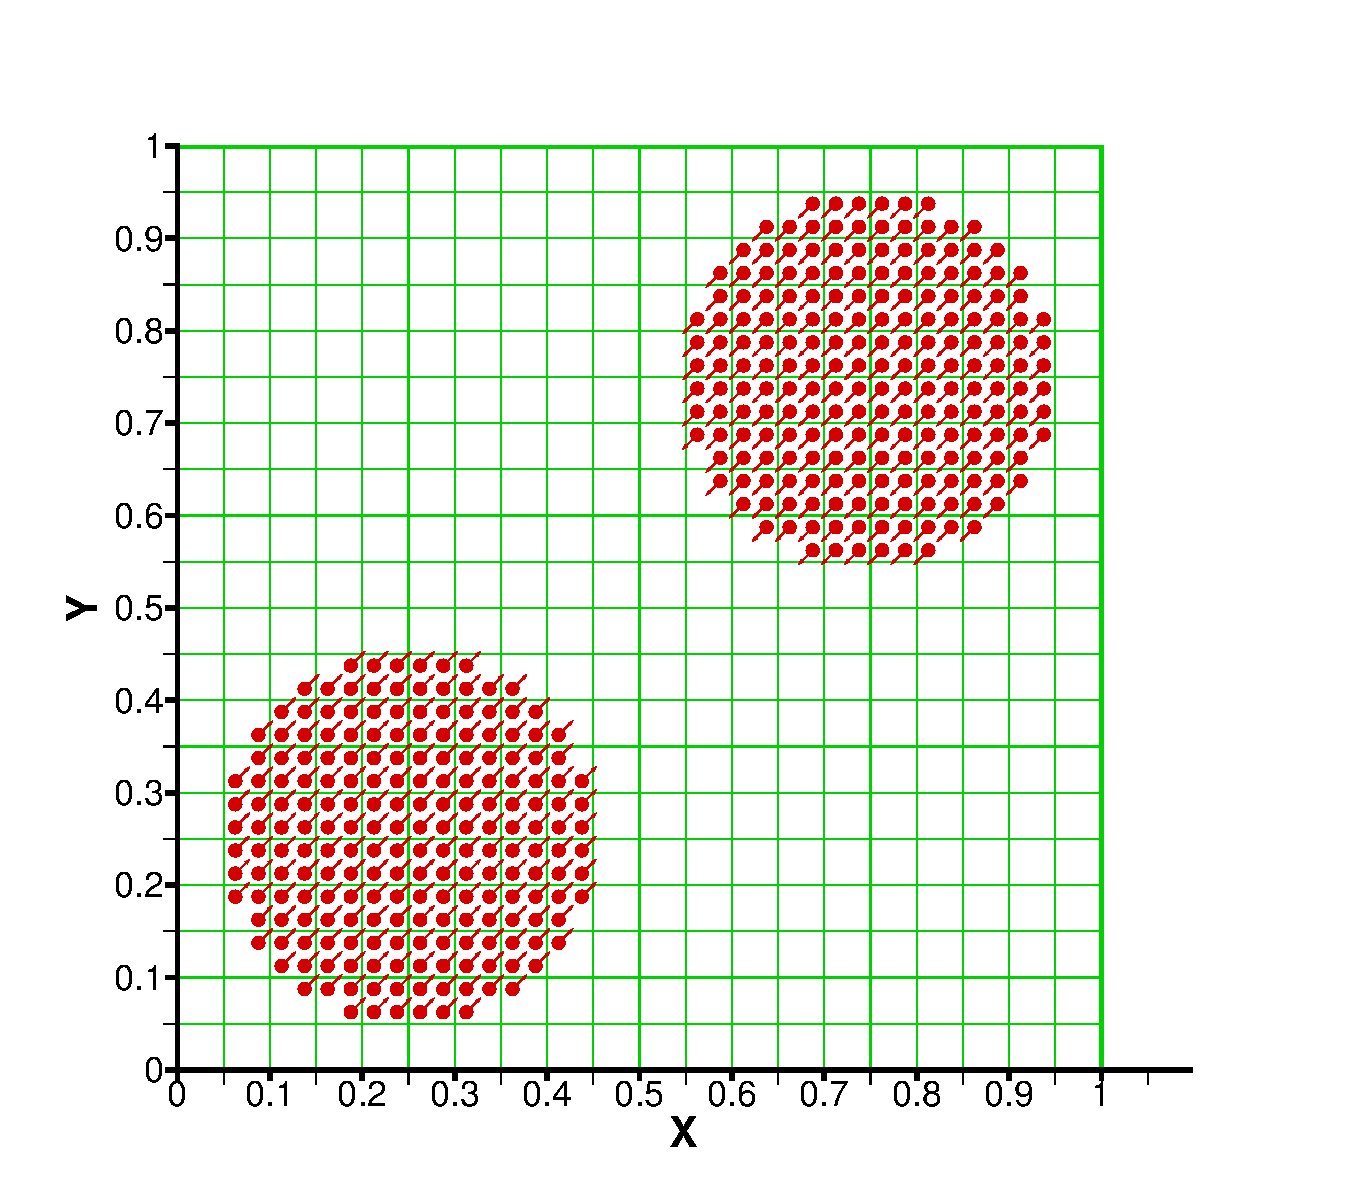
\includegraphics{Figures/disks.pdf}}
  %\epsfysize=3.5in
  %\epsfbox{Figures/disks.eps}
  \caption{\label{fig-disks_init} Initial particle representation of two
                                colliding disks on an overlying mesh.}
\end{figure}

The method usually uses a regular structured grid as a 
computational mesh.
While this grid, in principle, deforms as the material that it 
is representing
deforms, at the end of each timestep, it is reset to it's 
original undeformed
position, in effect providing a new computational grid for each 
timestep.
The use of a regular structured grid for each time step has a 
number of
computational advantages.  Computation of spatial gradients is 
simplified.
Mesh entanglement, which can plague fully Lagrangian techniques, 
such as
the Finite Element Method (FEM), is avoided.  MPM has also been 
successful
in solving problems involving contact between colliding objects, 
having an
advantage over FEM in that the use of the regular grid 
eliminates the
need for doing costly searches for contact surfaces\cite{bard}.

The choice of MPM over FEM as the C-SAFE structural mechanics method
was only in small part for the above mentioned criteria.  The
primary motivation was the ability to use MPM together with a multimaterial
CFD algorithm for solving tightly coupled fluid-structure interaction
problems.  This capability was first demonstrated in the CFDLIB
codes from Los Alamos by Bryan Kashiwa and co-workers.  There, as
in Uintah, MPM serves as the Lagrangian description of the solid
material in a multimaterial CFD code.  Certain elements of the
solution procedure are based in the Eulerian CFD algorithm, including
intermaterial heat and momentum transfer as well as satisfaction
of a multimaterial equation of state.  The use of a Lagrangian method
such as MPM to advance the solution of the solid material eliminates
the diffusion typically associated with Eulerian methods.

\section{Algorithm}

While a more detailed description of MPM can be found in 
\cite{sulskycpc},
the algorithm is laid out here.  The equations of motion are 
cast in the
form:

\begin{eqnarray}
	\tn{M}_g \cdot \tn{a}_g &=& \tn{Fext}_g - \tn{Fint}_g  
\label{newton2}
\end{eqnarray}
where $\tn{M}_g$ is the mass matrix, $\tn{a}_g$ is the 
acceleration vector,
$\tn{Fext}_g$ is the external force vector (sum of the body 
forces and
tractions), and $\tn{Fint}_g$ is the internal force vector 
resulting from
the divergence of the material stresses.  In general, $\tn{M}_g$ 
is a 
large, sparse matrix.  In practice, and in what follows here, a 
``lumped"
mass matrix is used, which only has entries on the diagonal, and 
is thus
represented as a column matrix.

The solution procedure begins by interpolating the particle 
state to the
grid, to form $\tn{M}_g$, $\tn{Fext}_g$, and to get a velocity 
on the grid
$\tn{v}_g$.  These quantities are calculated at each grid
node by the following equations:

\begin{eqnarray}
        \tn{M}_i &=& \sum_{p} S_{ip} m_p  
\label{expinterpolatemass}
\end{eqnarray}
\begin{eqnarray}
        \tn{v}_i &=& \frac{\sum\limits_{p} S_{ip} m_p 
\tn{v}_p}{\tn{M}_i} \label{expinterpolatevel}
\end{eqnarray}
\begin{eqnarray}
        \tn{Fext}_i &=& \sum_{p} S_{ip} \tn{Fext}_p. 
\label{expinterpolateFext}
\end{eqnarray}
$m_p$ is the particle
mass, $\tn{v}_p$ is the particle velocity, and $\tn{Fext}_p$ is 
the external
force on the particle.  The external force on the particle is 
generally an applied load of some type.  In Equation 
\ref{expinterpolatevel}, the numerator is the nodal momentum, 
which is then divided by the nodal mass to get a velocity.  
$S_{ip}$ is a ``shape function" for the $ith$ node
evaluated at $\tn{x}_p$.  Traditionally, the shape functions are 
multiplicative
combinations of one dimensional tent functions, as shown in
Figure \ref{fig-Sip}.  The shape functions serve to distance 
weight the contribution of each particle to the grid nodes.  

\begin{figure}[bh]
  \hspace{1.75in}
  \scalebox{0.7}{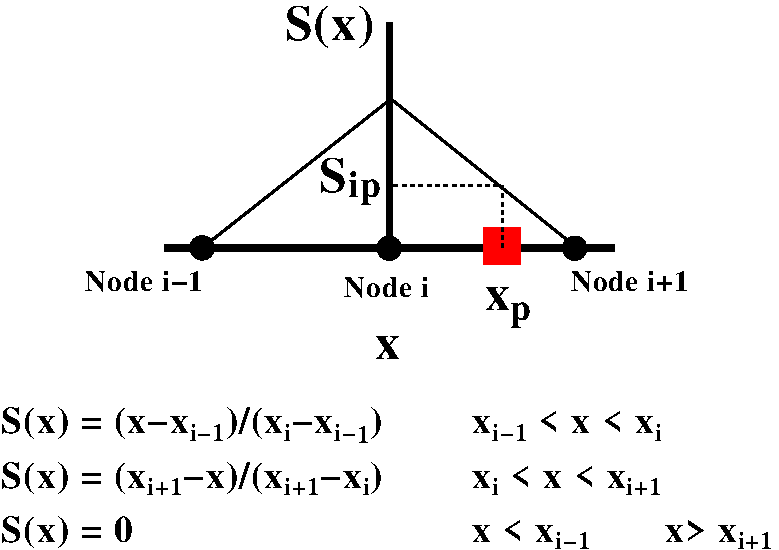
\includegraphics{Figures/Sip.pdf}}
  %\epsfysize=2.5in
  %\epsfbox{Figures/Sip.eps}
  \caption{\label{fig-Sip} One dimensional linear shape function, 
           $S(x)$.}
\end{figure}

At this point, a velocity gradient,  $\nabla \tn{v}_p$ is 
computed at
each particle using the grid velocities $\tn{v}_g$:

\begin{eqnarray}
	\nabla \tn{v}_p = \sum_i \tn{G}_{ip} \tn{v}_I
 \label{velgrad}
\end{eqnarray}

\noindent
where $\tn{G}_{ip}$ is the gradient of the $ith$ node's shape 
function,
evaluated at $\tn{x}_p$.  A one dimensional example of 
$\tn{G}_{ip}$ is
shown in Figure \ref{fig-Gip}.  Note that in going to multiple dimensions,
the $\tn{G}_{ip}$ are found by taking gradients of the multidimensional
$S_{ip}$ NOT by forming multiplicative combinations of the one-dimensional
$\tn{G}_{ip}$.

\begin{figure}[h]
  \hspace{1.75in}
  \scalebox{0.7}{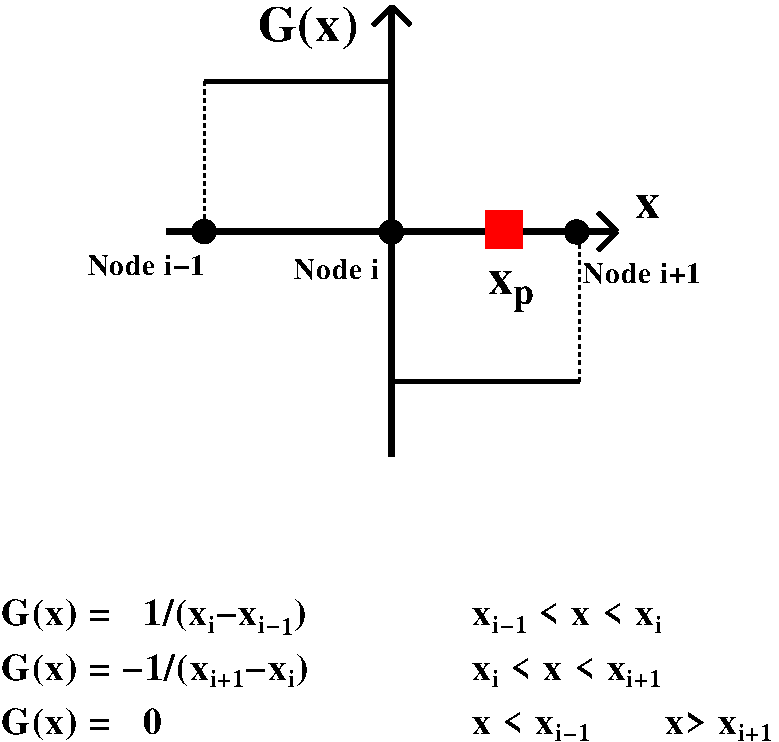
\includegraphics{Figures/Gip.pdf}}
  %\epsfysize=2.5in
  %\epsfbox{Figures/Gip.eps}
  \caption{\label{fig-Gip} One dimensional linear shape function 
           derivative, $G(x)$.}
\end{figure}
This velocity gradient is used as input to a constitutive model 
(stress-strain
relationship) which is evaluated at each particle.  The 
specifics of this 
calculation are dependent on the constitutive model.  An example 
of a simple elastic material model is described in the appendix.  
The result of this
calculation is the Cauchy stress at each particle, $\sig_p$.  
With this,
the internal force due to the divergence of the stress is 
calculated:

\begin{eqnarray}
	\tn{Fint}_g &=& \sum_{p} \tn{G}_{ip} \sig_p v_p
\end{eqnarray}

\noindent
where $v_p$ is the particle volume.  The internal force can be 
thought of as the force that holds a material together.  For a 
given deformation, this force is larger for stiffer materials.

Everything is now available to solve Equation \ref{newton2} for 
$\tn{a}_g$.
With that, the backward Euler method is used for all time 
integrations.
A convective grid velocity $\tn{v}^L_g$ is computed:

\begin{eqnarray}
	\tn{v}^L_g &=& \tn{v}_g  + \tn{a}_g dt
\end{eqnarray}

While the following calculation is never carried out, in 
principal, the
nodes of the grid also move with that convective velocity:

\begin{eqnarray}
	\tn{x}^L_g &=& \tn{x}_g  + \tn{v}^L_g dt     
\label{expdefgrid}
\end{eqnarray}

During this part of the computation, the particles move with the 
deforming
grid.  Their position and velocity is explicitly updated by:

\begin{eqnarray}
	\tn{v}_p (t + dt)  &=& \tn{v}_p (t)  + \sum_{i} S_{ip} 
\tn{a}_i  dt
\end{eqnarray}

\begin{eqnarray}
	\tn{x}_p (t + dt)  &=& \tn{x}_p (t)  + \sum_{i} S_{ip} 
\tn{v}^L_i  dt
\end{eqnarray}

This completes one timestep.  Note that not carrying out the 
calculation
in \ref{expdefgrid} explicitly has the effect of resetting the 
deformed
grid to it's undeformed position at the end of the timestep 
cycle.

As with all explicit time integration methods, a timestep size 
limit must
be enforced such that $dt < dx/(|\tn{v}_p| + c)$ for all 
particles, where $dx$ is the computational grid spacing and $c$ 
is the speed at which stress waves propagate through the 
material.
Failure to adhere to this condition will cause the solution to 
become
unstable and blow up.  The material wavespeed depends on the 
material model used, as well as on the particular parameters
chosen for that model.  Specifics of calculating the wavespeed
are given in the appendix.

\bibliographystyle{unsrt}
\bibliography{Bibliography}

\appendix
\section{Hyperelastic Material Models}

The subject of modeling the response of materials to deformation 
is a subject that has filled numerous textbooks.  Therefore, 
rather than attempt to condense these volumes, here the reader 
will be simply be given a simple material response model.  Other 
more complex material response models can be interchanged in the 
framework discussed above quite readily.

The author has come to prefer a class of models known as 
hyperelastic models.  What this means is that the stress 
response of these materials is derived from a strain energy 
function.  A strain energy function gives a relationship between 
the state of deformation that a material is in, and the amount 
of stored strain energy that this material has.  This is akin to 
the familiar relationship for the stored energy in a spring, 
$W=\frac{1}{2} k dx^2$ where k is the spring constant, and $dx$ is
the distance that the spring has been compressed or extended.

One such strain energy function is given by:

\begin{eqnarray}
	W &=& \frac{\lambda}{4}(J^2-1)
 - (\frac{\lambda}{2}+\mu) lnJ
+ \frac{\mu}{2}(trace(\tn{F}^T\tn{F} - 3)
\end{eqnarray}

from which the following relationship for the stress can be 
derived:

\begin{eqnarray}
       \sig &=& \frac{\lambda}{2}(J-\frac{1}{J})\tn{I} 
  + \mu (\tn{F}\tn{F}^T) - \tn{I})
 \label{stress}
\end{eqnarray}

where $\lambda$ and $\mu$ are material constants, while $J$ and 
$\tn{F}$ describe the state of deformation.  These will be 
defined shortly.

In the Algorithm section, the calculation of the velocity 
gradient, $\nabla \tn{v}_p$ is given in Equation \ref{velgrad}.
Starting from there, we can then compute an increment in the 
deformation gradient, $\tn{F}(dt)$ by:
\begin{eqnarray}
	\tn{F}(dt) &=& \nabla \tn{v}_p dt + \tn{I}.
\end{eqnarray}
This increment in the deformation gradient can then be used to 
compute a new total deformation gradient using:
\begin{eqnarray}
	\tn{F}(t+dt) &=& \tn{F}(dt) \tn{F}(t).
\end{eqnarray}
Note that the initial (t=0) deformation gradient is simply the 
identity, i.e. $\tn{F}(0) = \tn{I}$.  Now with the deformation 
gradient, one can compute $J$ by:
\begin{eqnarray}
	J &=& det(\tn{F}(t+dt)).
\end{eqnarray}

Note that $J$ represents the volumetric part of the deformation.  
Specifically, it is the ratio of the current volume of an 
element of material to it's original volume.  Similarly, we can
define an increment in $J$ as:
\begin{eqnarray}
	J_{inc} &=& det(\tn{F}(dt))
\end{eqnarray}
which  is the ratio of the current volume of an element of 
material to it's volume at the previous timestep.  Thus we can 
write:
\begin{eqnarray}
	v_p(t+dt) &=& J_{inc} v_p(t).
\end{eqnarray}

Elastic material properties are frequently given in terms of 
bulk and shear moduli, or $\kappa$ and $\mu$.  The shear is 
sometimes denoted by $G$.  The shear modulus $\mu$ appears in 
Equation \ref{stress} above.  $\lambda$ can be computed from
$\kappa$ and $\mu$ by:
\begin{eqnarray}
	\lambda &=& \kappa - \frac{2}{3}\mu.
\end{eqnarray}

Lastly, based on material properties $\lambda$ and $\mu$, a material 
wavespeed can be computed:

\begin{eqnarray}
	c^2 &=& (\lambda + 3 \mu)\frac{m_p}{v_p}.
\end{eqnarray}

This wavespeed can be used in computing the timestep size as 
described above.

\section{Other Material Models In the UCF}
Other material models implemented into the Uintah Computational
Framework (UCF) have been chosen for three purposes:
\begin{itemize}
  \item To verify the accuracy of the material point method (MPM)
        and to validate the coupling between the computational fluid 
        dynamics code (ICE) and MPM.
  \item To model the elastic-plastic deformation of the steel
        container and the consequent damage in the regimes of 
        both high and low strain rates and high and low temperatures.
  \item To model the polymer bonded explosive contained in the 
        container under various strain rates and temperatures.
\end{itemize}

\subsection{Material models for the validation of MPM}
The models that have been implemented for the verification of MPM
are:
\begin{itemize}
   \item Isotropic hypoelastic model using the Jaumann rate of 
         stress.
     \begin{enumerate}
        \item  MPM predictions have been compared with exact results 
               for thick cylinders under internal pressure for small
               strains, three-point beam bending, etc.
        \item  MPM predictions for the strain/stress contours for
               a set of disks in contact have been found to match
               experimental results.
     \end{enumerate}
   \item Isotropic hyperelastic material models for Mooney-Rivlin
         rubber and a modified compressible Neo-Hookean material. 
         Isotropic strain hardening plasticity for the Neo-Hookean
         material.
     \begin{enumerate}
        \item  A billet compression problem has been simulated using
               MPM and the results have been found to closely 
               match finite element simulations.
        \item  MPM simulations for a thick cylinder under internal
               pressure with plastic deformation (perfect plasticity)
               compare well with the exact solution.
     \end{enumerate}
\end{itemize}

\subsection{Material models for the container}
The material model for the steel container is used to determine
the state of stress in the container for an applied deformation
rate and deformation gradient at each material point.  The strain 
rates can vary from $10^{-3}$/s to $10^6$/s and temperatures in 
the container can vary from 250 K to 1000 K.  Plasticity dominates
the deformation of the container during the expansion of the 
explosive gases inside.  At high strain rates the volumetric
response of the container is best obtained using an equation of 
state.  After the plastic strain in the container
has reached a threshold value a damage/erosion model is required to
rupture the container.

Two plasticity models with strain rate and temperature dependency 
are the Johnson-Cook and the Mechanical Threshold Stress (MTS) 
models.  The volumetric response is calculated using a modified
Mie-Gruneisen equation of state.  A damage model that ties in well 
with the Johnson-Cook plasticity model is the Johnson-Cook damage 
model.  The erosion algorithm either removes the contribution
of the mass of the material point or forces the material point
to undergo no tension or shear under further loading.

The stress update at each material point is performed using either
of the two methods discussed below.
\begin{itemize}
   \item Isotropic Hypoelastic-plastic material model using an 
         additive decomposition of the rate of deformation tensor.
     \begin{enumerate}
        \item The rate of deformation tensor a material point
              is calculated using the grid velocities.
        \item An incremental update of the left stretch and the
              rate of rotation tensors is calculated.
        \item The stress and the rate of deformation are rotated
              into the material coordinates.
        \item A trial elastic deviatoric stress state is calculated.
        \item The flow stress is calculated using the plasticity
              model and compared with the vonMises yield condition.
        \item If the stress state is elastic, an update of the 
              stress is computed using the Mie-Gruneisen equation
              of state or the isotropic hypoelastic constitutive
              equation.
        \item If the stress state is plastic, all the strain rate 
              is considered to the plastic and an elastic correction
              along with a radial return step move the stress state
              to the yield surface.  The hydrostatic part of the 
              stress is calculated using the equation of state or
              the hypoelastic constitutive equation.
        \item A scalar damage parameter is calculated and used
              to determine whether material points are to be eroded
              or not.
        \item Stresses and deformation rates are rotated back to the
              laboratory coordinates.
     \end{enumerate}
   \item Isotropic Hyperelastic-plastic material model using a 
         multiplicative decomposition of the deformation gradient.
     \begin{enumerate}
        \item The velocity gradient at a material point
              is calculated using the grid velocities.
        \item An incremental update of the deformation gradient and
              the left Cauchy-Green tensor is calculated.
        \item A trial elastic deviatoric stress state is calculated
              assuming a compressible Neo-Hookean elastic model.
        \item The flow stress is calculated using the plasticity
              model and compared with the vonMises yield condition.
        \item If the stress state is elastic, an update of the 
              stress is computed using the Mie-Gruneisen equation
              of state or the compressible Neo-Hookean constitutive
              equation.
        \item If the stress state is plastic, all the strain rate 
              is considered to the plastic and an elastic correction
              along with a radial return step move the stress state
              to the yield surface.  The hydrostatic part of the 
              stress state is calculated using the Mie-Gruneisen
              equation of state or the Neo-Hookean model.
        \item A scalar damage parameter is calculated and used
              to determine whether material points are to be eroded
              or not.
     \end{enumerate}
\end{itemize}

The implementations have been tested against Taylor impact test data
for 4340 steel and HY 100 steel as well as one-dimensional problems
which have been compared with experimental stress-strain data.  At 
large tensile strains, material points tend to separate from the 
main body.  This issue is currently being explored and solutions are
being sought in the framework of MPM.

\subsection{Material models for the explosive}
The explosive is modeled using the ViscoSCRAM constitutive 
model.  Since large deformations or strains are not expected in 
the explosive, a small strain formulation has been implemented into 
the UCF.  The model consists of five generalized Maxwell elements
arranged in parallel, crack growth, friction at the crack 
interfaces and heating due to friction and reactions at the 
crack surfaces.  The implementation has been verified with 
experimental data and found to be accurate.

\end{document}

